\documentclass[11pt, oneside]{article}   	% use "amsart" instead of "article" for AMSLaTeX format
\usepackage{geometry}                		% See geometry.pdf to learn the layout options. There are lots.
\geometry{letterpaper}                   		% ... or a4paper or a5paper or ... 
%\geometry{landscape}                		% Activate for rotated page geometry
\usepackage[parfill]{parskip}    			% Activate to begin paragraphs with an empty line rather than an indent
\usepackage{graphicx}				% Use pdf, png, jpg, or eps§ with pdflatex; use eps in DVI mode
								% TeX will automatically convert eps --> pdf in pdflatex		
\usepackage{amssymb}
\usepackage{mathtools}
\usepackage{enumerate}
\usepackage{tikz}
\usepackage{listings}
\usetikzlibrary{arrows}
\usepackage{graphicx}
\usepackage{caption}
\usepackage{subcaption}
\usepackage{amsmath}
\usepackage{commath}
\usepackage{physics}
\usepackage{float}
\usepackage{color,soul}

\def\firstcircle{(90:1.75cm) circle (2.5cm)}
\def\secondcircle{(210:1.75cm) circle (2.5cm)}
\def\thirdcircle{(330:1.75cm) circle (2.5cm)}
\geometry{left=2.5cm,right=2.5cm,top=2.5cm,bottom=2.5cm}
%SetFonts

%SetFonts


\title{Removing Blur \& Multiplicative Noise Using Convex Optimization}
\author{Pushen Wang, Jimmy Ye}

\date{March, 2017}							% Activate to display a given date or no date

\begin{document}

\maketitle

\section{Abstract}

A common problem in signal processing is recovering the true signal from a
noise-corrupted signal. We consider a specific domain of this general problem,
multiplicative noise and blurring in images. Both are common in images due to
sensor imperfections, shadows, motion, poor focus, etc. In particular, we would
like to find a model which captures properties of a less noisy image and is
amenable to computationally efficient methods of convex optimization. Since it
is usually impossible to recover the true image, the models and approaches are
evaluated by how well they recover significant details like edges, whether they
introduce additional artifacts, and their efficiency in terms of time
complexity.

\section{Introduction}

Suppose that an imaging system captures an image which is distorted by blurring
and multiplicative noise. This process could be described as:
\begin{equation} \label{eqn:formulation}
u_0 = (Au)\eta
\end{equation}
where $u$ is the ``true'' image, $A$ is a blurring operator and $\eta$ is a
multiplicative noise. The problem is to restore the original image $u$ from the
degraded image $u_0$, and the recovering process is called de-blurring
and de-noising.

Different constraints may be placed on blurring operator $A$ and multiplicative
noise $\eta$ in different applications. For example, $\eta$ follows a Gamma
distribution in synthetic aperture radar(SAR), and follows a Rayleigh
distribution in ultrasound imaging, and when $A$ is the identity matrix, this
problem will degrade into multiplicative removal only.

Historically, it was common to use least-squares, i.e. $L_2$ norm, as the
optimization objective, however, it has been found that the total variation (TV)
norm, which is essentially $L_1$ norm of the derivative, is better \cite{rudin1992}.
We consider how to formulate multiplicative noise and blurring, using the TV
objective, as a computationally efficient optimization problem.

\section{Basic Formulation}

We first consider additive noise as a simpler problem before extending the
optimization problem to multiplicative noise and blurring. As in \cite{rudin1992}, we
denote the pixel values of a noisy image, or the observed intensity function,
$u_0(x,y)$, the desired denoised image as $u(x,y)$, and the additive noise as
$n$. Then we have
\begin{equation}
  u_0(x,y) = u(x,y) + n(x,y)
\end{equation}

The total variation norm for a function with domain $[a,b]$ is defined as
\begin{equation}
  V(f) = \sup_P \sum_{i=1}^{n_p - 1} \abs{f(x_{i+1}) - f(x_i)}
\end{equation}
where $P$ is the set of all partitions $p = \{x_0,...,x_{n_p}\}$ of the domain.

This definition can be extended to an $n$-dimensional $\Omega$:
\begin{equation}
  V(f, \Omega) = \sup \{\int_{\Omega}f(x) (\nabla \cdot \phi (x)) \dd{x} : \phi \in C_c^1(\Omega), \norm{\phi}_{L^\infty(\Omega)} \leq 1 \}
\end{equation}
where $C_c^1(\Omega)$ denotes the space of continuously differentiable functions
with compact support (i.e. in $\Omega \subset \mathbb{R}^n$, $f$ is nonzero only
on a bounded set) and the norm used is supremum on sets of nonzero measure.

The following theorem gives a more manageable definition:
\begin{equation}
  V(f) = \int_{\Omega} \norm{\nabla f(x)}_2 dx
\end{equation}

Now we have our optimization problem \cite{rudin1992}:
\begin{align}
  \text{minimize} &\int_\Omega \sqrt{u_x^2 + u_y^2} \dd{x} \dd{y} \\
  \text{subject to} &\int_\Omega (u - u_0) \dd{x} \dd{y} = 0 \\
                    &\int_\Omega \frac{1}{2} (u - u_0)^2 \dd{x} \dd{y} = \sigma^2
\end{align}
Here, $u_x$ and $u_y$ are the partial derivatives of $u$, and the constraints
enforce our simplifying assumption that the additive noise follows a Gaussian
distribution with mean zero and standard deviation $\sigma$. Note that
$\norm{\nabla f(x)}_2 = \sqrt{u_x^2 + u_y^2}$.

However, this problem is optimizing over a function of $u$, which is itself a
function. We can apply the Euler-Lagrange equations to obtain a PDE, a form more
amenable to numerical solutions, which when satisfied gives us the desired $u$
which optimizes TV \cite{rudin1992}:
\begin{align}
  0 &= \pdv{}{x} \Bigg(\frac{u_x}{\sqrt{u_x^2+u_y^2}} \Bigg) +
  \pdv{}{y} \Bigg(\frac{u_y}{\sqrt{u_x^2+u_y^2}} \Bigg) - v_1 - v_2(u - u_0) \text{ on } \Omega, \text{with} \\
  \pdv{u}{n} &= 0 \text{ on } \partial \Omega, \text{the boundary of } \Omega
\end{align}

We solve numerically by introducing an additional time parameter, optimizing
$u(x,y,t)$ \cite{rudin1992}:
\begin{align}
  u_t &= \pdv{}{x} \Bigg(\frac{u_x}{\sqrt{u_x^2+u_y^2}} \Bigg) +
  \pdv{}{y} \Bigg(\frac{u_y}{\sqrt{u_x^2+u_y^2}} \Bigg) - v(u - u_0) \text{ for } t > 0 \\
  \pdv{u}{n} &= 0 \text{ on } \partial \Omega, \text{the boundary of } \Omega
\end{align}
where $u(x,y,0)$ is given. Note that the mean constraint is satisfied so long as
$u(x,y,0)$ has the same mean as $u_0$.

We compute $v(t)$ by multiplying both sides of the previous equation by $(u -
u_0)$ and integrating by parts \cite{rudin1992}:
\begin{equation}
  v = - \frac{1}{2\sigma^2} \int \Bigg[ \sqrt{u_x^2 + u_y^2} -
  \Bigg( \frac{(u_0)_xu_x}{\sqrt{u_x^2+u_y^2}} +
  \frac{(u_0)_yu_y}{\sqrt{u_x^2+u_y^2}} \Bigg) \Bigg] \dd{x} \dd{y}
\end{equation}

This is essentially Rosen's gradient projection method \cite{rudin1992}, a
variation of gradient descent that takes at each step, the projection of $-
\nabla f$ onto the feasible set, instead of $- \nabla f$ itself, as the
increment, and is therefore applicable to constrained optimization problems.

Thus, by taking the appropriate numerical approximations of $u_t$ and $v(t)$, we
have a completely specified numerical algorithm for optimizing $u$ in the case
of Gaussian-distributed additive noise.

\section{Multiplicative Noise \& Deblurring}

We can account for multiplicative noise and blurring (formulation is given by (\ref{eqn:formulation})) by modifying our
constraints, which then affects the last terms of $u_t$, but the core idea,
including the optimization algorithm, remains the same.

The new constraints \cite{rudin2003}:
\begin{align}
  &\int_\Omega \Bigg(\frac{u_0(x,y)}{Au(x,y)} \Bigg) \dd{x} \dd{y} = 1 \\
  &\int_\Omega \Big(\frac{u_0}{Au} - 1 \Big)^2 \dd{x} \dd{y} = \sigma^2
\end{align}
which are still under the assumption that the noise $\eta$ is
Gaussian-distributed, but since it is multiplicative, it now has mean 1. Note
also the introduction of the blurring term $A$, a linear convolution operator
(transforming matrices / 2D functions rather than vectors / 1D functions).

The new $u_t$ \cite{rudin2003}:
\begin{equation}
  u_t = \pdv{}{x} \Bigg(\frac{u_x}{\sqrt{u_x^2+u_y^2}} \Bigg)
  + \pdv{}{y} \Bigg(\frac{u_y}{\sqrt{u_x^2+u_y^2}} \Bigg)
  - v_1A^*\Bigg(\frac{u_0}{(Au)^2} \Bigg) \Big(\frac{u_0}{Au} \Big)
  - v_2A^*\frac{u_0}{(Au)^2}
\end{equation}
where $A^*$ is the adjoint operator of $A$ (intuitively, a sort of dual operator
which generalizes the idea of the complex conjugate of a complex number, or the
conjugate transpose of a matrix).

We have shown that it is possible, with minimal additions and modifications, to
extend our numerically solvable additive noise model to a model which
simultaneously captures multiplicative noise and convolutional blurring.

Figure \ref{fig:noisy} is the result of a Gaussian blur with $\sigma^2 = 2$ and
multiplicative noise with $\sigma = 0.2$ applied to the original Figure
\ref{fig:original}, and Figure \ref{fig:denoised} shows the result of the
total variation based algorithm in \cite{rudin2003}:
\begin{figure}
    \centering
    \begin{subfigure}[b]{0.3\textwidth}
        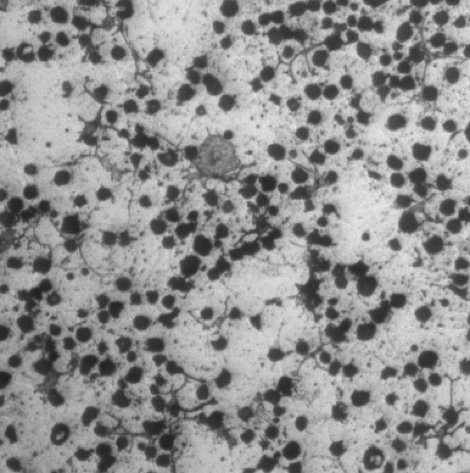
\includegraphics[width=\textwidth]{figure/original}
        \caption{Original image}
        \label{fig:original}
    \end{subfigure}
    \begin{subfigure}[b]{0.3\textwidth}
        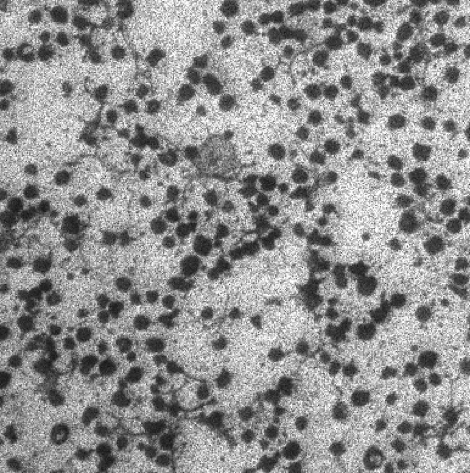
\includegraphics[width=\textwidth]{figure/noisy}
        \caption{Noisy image}
        \label{fig:noisy}
    \end{subfigure}
    \begin{subfigure}[b]{0.3\textwidth}
        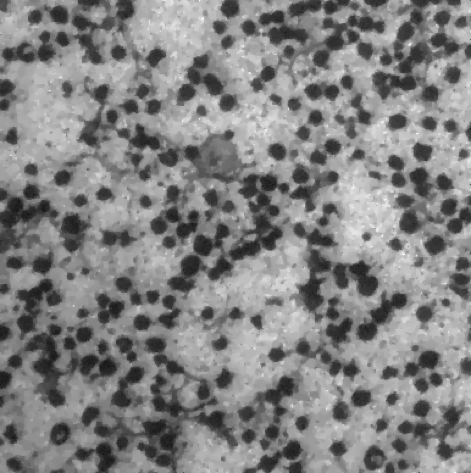
\includegraphics[width=\textwidth]{figure/denoised}
        \caption{Denoised image}
        \label{fig:denoised}
    \end{subfigure}
    \caption{Experiment results given in \cite{rudin2003}}\label{fig:result}
\end{figure}

\section{Advanced Techniques}

There are some additional improvements we can make to the quality of our
denoised images as well as the efficiency of our algorithm. In particular, we
can find a convex approximation to our nonconvex problem, which guarantees a
good global optimum, rather than simply assuming local near-convexity to achieve
good local optimums. We can then apply a different optimization algorithm, the
alternating direction method of multipliers (ADMM), which outputs better images
and is generally at least an order of magnitude faster \cite{wang2013fast}.

The basic idea given in \cite{wang2013fast} is to transform the multiplicative
noise to additive noise through a logarithm:
$$\log u_0 = \log Au + \log \eta$$
And then similar to the previous approach, based on total variation, this
problem can be formulated as:
\begin{align}
  \text{minimize } & ||\nabla u||_1 \\
  \text{subject to } & u \in \mathbb{R}^n \\
                    & || \log u_0 - \log Au ||_1 \leq \alpha,
\end{align}
where $n$ is the number of pixels, $\alpha$ is the trade-off between the fit to
$f$ and the amount of regularization, and $||\cdot||_1$ is $L_1$-norm.

\bibliographystyle{plain}
\nocite{*}
\begin{thebibliography}{3}

\bibitem{rudin1992}
Leonid~I Rudin, Stanley Osher, and Emad Fatemi.
\newblock Nonlinear total variation based noise removal algorithms.
\newblock {\em Physica D: Nonlinear Phenomena}, 60(1-4):259--268, 1992.

\bibitem{rudin2003}
Leonid Rudin, Pierre-Luis Lions, and Stanley Osher.
\newblock Multiplicative Denoising and Deblurring: Theory and Algorithms.
\newblock {\em Multiplicative Denoising and Deblurring: Theory and Algorithms}, 2003.

\bibitem{wang2013fast}
Fan Wang and Michael~K Ng.
\newblock A fast minimization method for blur and multiplicative noise removal.
\newblock {\em International Journal of Computer Mathematics}, 90(1):48--61,
  2013.

\end{thebibliography}
\end{document}